\subsection{Présentation de l'entreprise}
    Forssea Robotics est une jeune entreprise innovante en matière de robotique sous-marine. Elle propose des solutions industrielles à l'exploration de ce milieu particulièrement hostile à l'homme. Ils excellent principalement dans les quatre domaines suivants robotique autonome, ingénierie des \gls{ROV}s, vision sous-marine et intelligence artificielle, ce qui leur vaut de travailler aux côtés de nombreux partenaires, comme le groupe Total, Thales, iXblue, DeepOcean, et bien d'autres, mais aussi des centre de recherches comme l'\gls{ENSTAB}.

\subsection{Présentation des produits}
    Forssea Robotics propose deux \gls{ROV}s\footnote{\url{https://forssea-robotics.fr/index.php/products/rovs}} : \textsc{Argos} et \textsc{Atoll}. Ces robots permettent d'effectuer des missions dans le milieu sous-marin. \gls{Argos} est présenté comme un robot d'intervention léger intelligent permettant d'embarquer une charge utile pesant jusqu'à $30\ kg$ et pouvant aller à une profondeur de $500\ m$ et même jusqu'à $2000\ m$ avec quelques modifications. \gls{Atoll} est quand à lui un robot de levage autonome. Il permet de déplacer et de positionner des \gls{frameLBL} sur les fonds marins. Il permet d'aller jusqu'à $3000\ m$ et de porter jusqu'à $1500\ kg$. Le \textsc{docking} sur la structure est quand à lui complètement autonome et basé sur des techniques de positionnement visuels.

    \begin{figure}[!htb]
        \centering
        \begin{subfigure}[b]{0.45\textwidth}
            \centering
            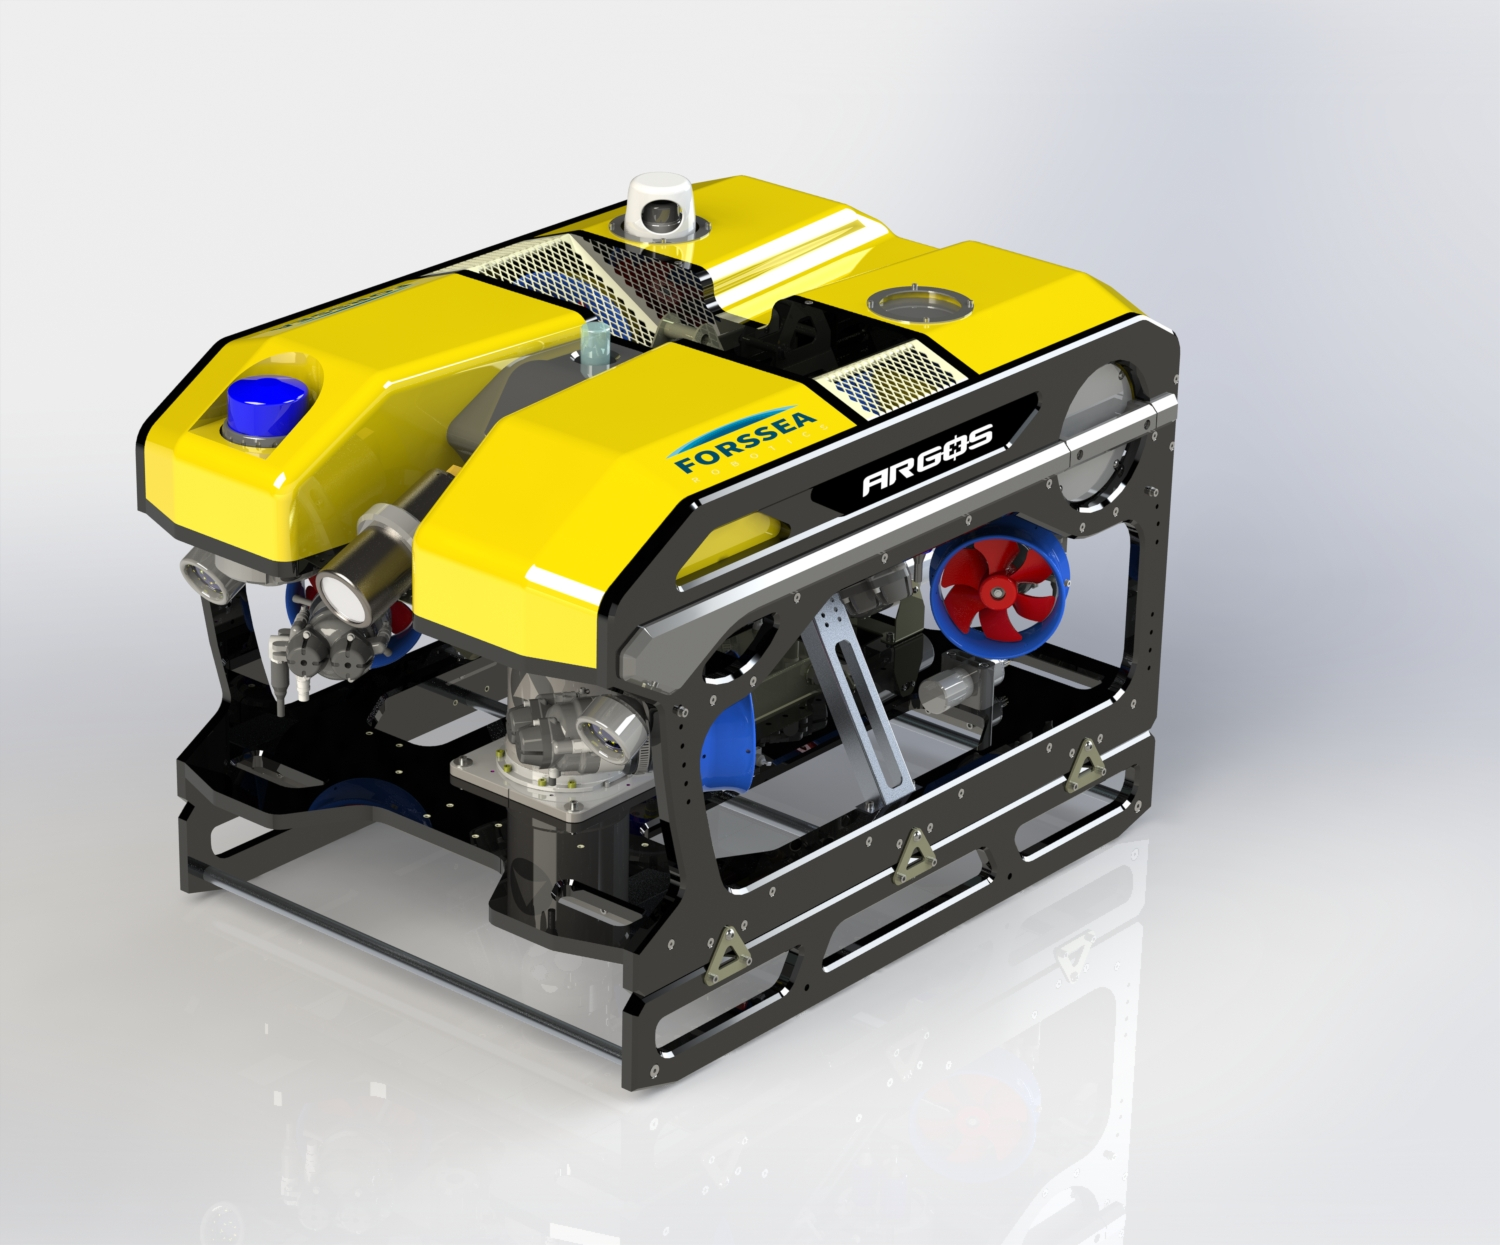
\includegraphics[width=\textwidth]{imgs/Argos.jpg}
            \caption{\gls{Argos}}
        \end{subfigure}
        \hfill
        \begin{subfigure}[b]{0.45\textwidth}
            \centering
            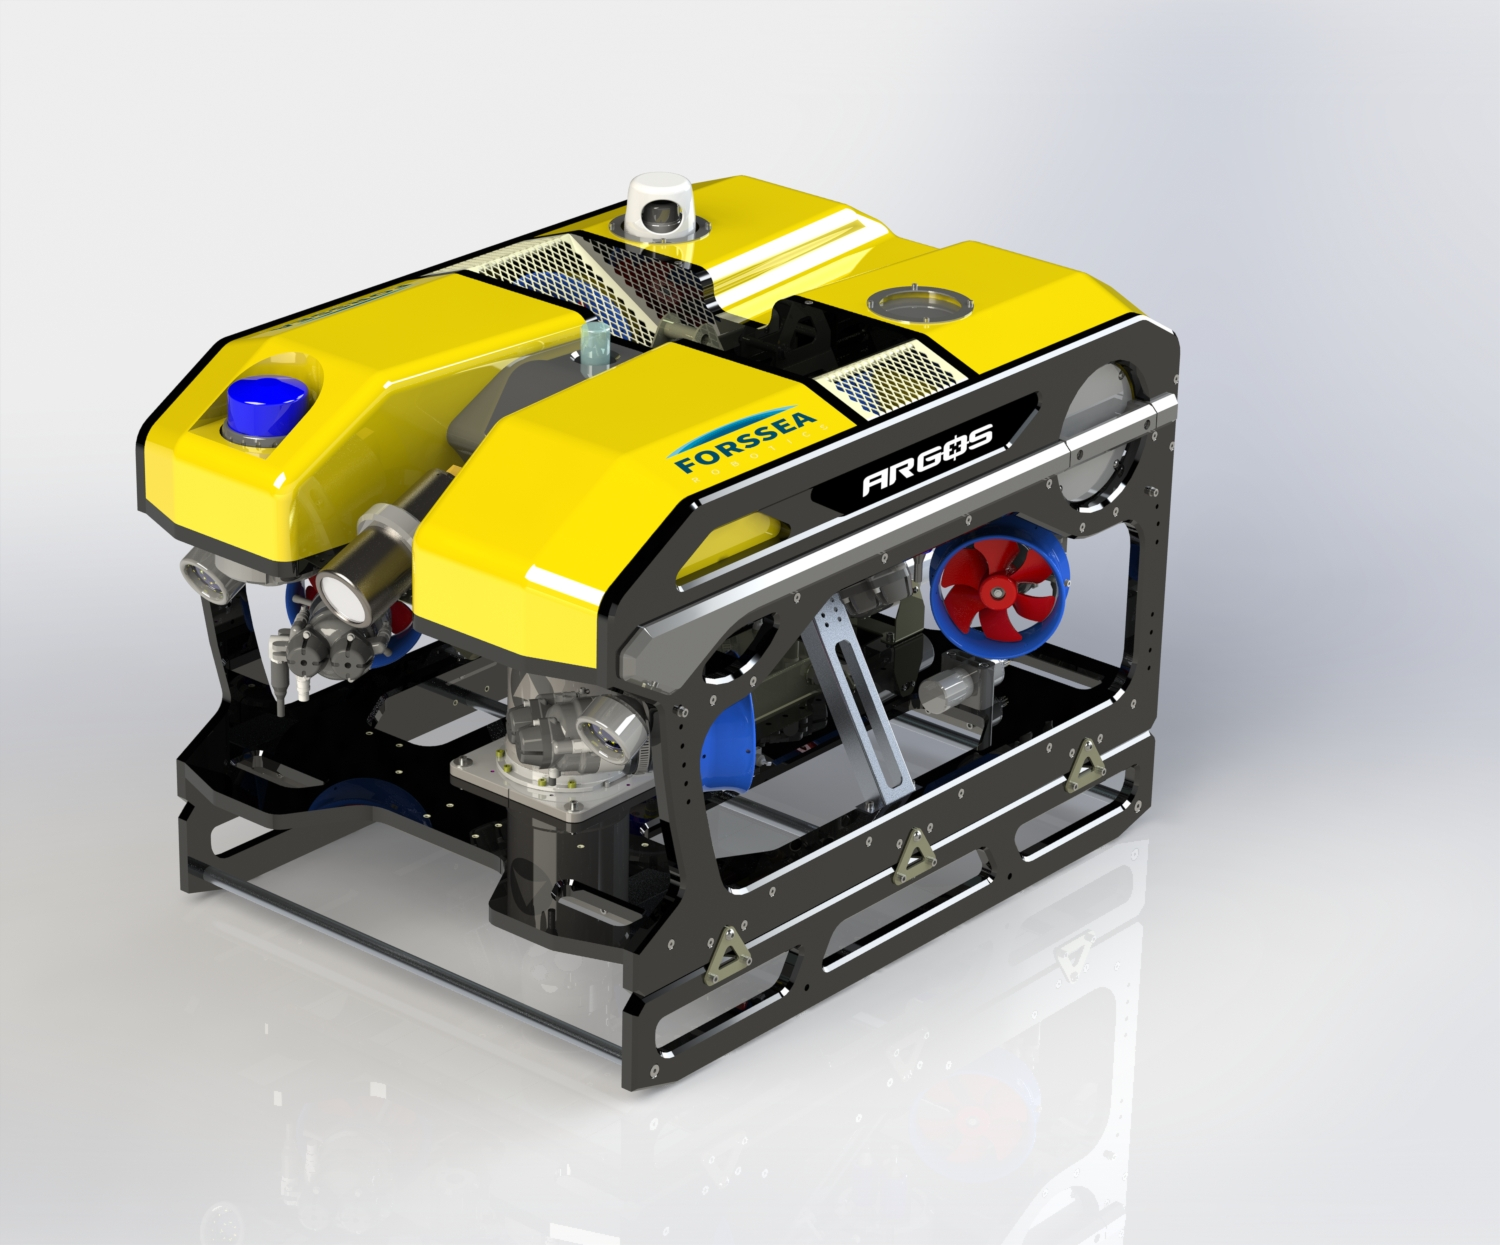
\includegraphics[width=\textwidth]{imgs/Argos.jpg}
            \caption{\gls{Atoll}}
        \end{subfigure}
        \caption{\gls{ROV}s proposés par Forssea Robotics}
    \end{figure}

    Ils proposent aussi plusieurs solutions de captations visuelles\footnote{\url{https://forssea-robotics.fr/index.php/products/cameras}}. Il y a la \gls{Navcam} qui est une caméra embarquant des algorithmes de traitement permettant de réaliser du positionnement visuel, et l'\gls{Obscam} qui est une simple caméra étanche.